% ============================================================
%  IoT Project Report Template
%  Compile with: pdflatex (run twice so the contents/lists update)
%  LOGO: put your college logo in the same folder as this file
%        and name it  college_logo.png  (or change \logofile below).
%        If the file is missing, a labelled empty box is shown instead.
% ============================================================
\documentclass[12pt,a4paper]{report}

\usepackage[a4paper,left=1.5in,right=1in,top=1in,bottom=1in]{geometry}
\usepackage{graphicx}
\usepackage{booktabs}
\usepackage{longtable}
\usepackage{tabularx}
\usepackage{array}
\usepackage{setspace}
\usepackage{fancyhdr}
\usepackage{listings}
\usepackage{xcolor}
\usepackage{caption}
\usepackage[hidelinks]{hyperref}

\onehalfspacing
\emergencystretch=3em

% ---------- FILL THESE IN ----------
\newcommand{\projecttitle}{AERIS: Aviation Experimental Recording and Instrumentation System}
\newcommand{\studentnames}{Manasvi Rathore (Roll No.\ 50)\\Pooja Lingwat (Roll No.\ 42, PRN 1262242831)\\Anjali Tripathi (Roll No.\ 40)}
\newcommand{\guidename}{Prof.\ Niyamat Ujloomwale}
\newcommand{\hodname}{Dr.\ B. M. Patil}
\newcommand{\department}{Department of Computer Science and Engineering}
\newcommand{\collegename}{School of Computer Science and Engineering}
\newcommand{\universityname}{MIT World Peace University (MIT-WPU), Pune}
\newcommand{\degreename}{Bachelor of Technology}
\newcommand{\academicyear}{2026--2027}
\newcommand{\logofile}{logo.png}
\newcommand{\rupee}{Rs.}  % currency label used in the BOM
% -----------------------------------

% Logo: shows the image if present, otherwise an empty box
\newcommand{\collegelogo}[1]{%
  \IfFileExists{\logofile}%
    {\includegraphics[height=#1]{\logofile}}%
    {\fbox{\parbox[c][#1][c]{#1}{\centering\small Place college\\logo here}}}%
}

% Code listing style
\lstset{basicstyle=\ttfamily\footnotesize,breaklines=true,frame=single,
        numbers=left,numberstyle=\tiny,backgroundcolor=\color{gray!8}}

% Header/footer
\pagestyle{fancy}
\fancyhf{}
\fancyhead[L]{\small AERIS IoT Project Report}
\fancyhead[R]{\small\department}
\fancyfoot[C]{\thepage}
\renewcommand{\headrulewidth}{0.4pt}

% Make chapter pages keep the footer page number
\fancypagestyle{plain}{\fancyhf{}\fancyfoot[C]{\thepage}\renewcommand{\headrulewidth}{0pt}}

\begin{document}

% ============================================================
%  FRONT MATTER
% ============================================================
\pagenumbering{roman}

% ---------------- TITLE PAGE ----------------
\begin{titlepage}
\thispagestyle{empty}
\centering
{\Large\bfseries \universityname\par}
\vspace{0.4cm}
{\Large\bfseries \collegename\par}
\vspace{0.3cm}
{\large \department\par}
\vspace{0.8cm}

\collegelogo{3.2cm}\par
\vspace{1cm}

{\large A Project Report on\par}
\vspace{0.4cm}
{\LARGE\bfseries \projecttitle\par}
\vspace{0.8cm}

{\large Submitted in partial fulfilment of the requirements for the degree of\par}
{\large\bfseries \degreename\par}
\vspace{0.8cm}

{\large Submitted by\par}
\vspace{0.3cm}
{\large\bfseries \studentnames\par}
\vspace{0.8cm}

{\large Under the guidance of\par}
{\large\bfseries \guidename\par}
\vfill
{\large Academic Year \academicyear\par}
\end{titlepage}

% ---------------- CERTIFICATE ----------------
\newpage
\thispagestyle{empty}
\begin{center}
\collegelogo{2.4cm}\par\vspace{0.4cm}
{\Large\bfseries \collegename\par}
{\large \department\par}
\vspace{1cm}
{\Large\bfseries CERTIFICATE\par}
\end{center}
\vspace{0.8cm}

\noindent This is to certify that the project report entitled
\textbf{``\projecttitle''} is a bonafide work carried out by

\begin{center}
\textbf{\studentnames}
\end{center}

\noindent in partial fulfilment of the requirements for the award of the degree of
\textbf{\degreename} in \textbf{\department} of \textbf{\universityname}
during the academic year \textbf{\academicyear}, under my supervision and guidance.

\vspace{2.2cm}
\noindent
\begin{tabularx}{\textwidth}{XXX}
\rule{4cm}{0.4pt} & \\
\textbf{\guidename}\\
Project Guide & \\
\end{tabularx}

\vspace{1.5cm}
\noindent Date: \hrulefill \\[0.3cm]
Place: \hrulefill

% ---------------- DECLARATION ----------------
\chapter*{Declaration}
\addcontentsline{toc}{chapter}{Declaration}
We hereby declare that the project report entitled \textbf{``\projecttitle''} has been prepared by us under the guidance and supervision of \guidename. We confirm that:
\begin{enumerate}
\item The hardware design, the STM32 and ESP8266 firmware and the dashboard software of AERIS are based on the open AERIS repository (\url{https://github.com/Quixotic1762/AERIS}) by Ashwin Kumar and Anvi Singh Parihar, which we used with their knowledge and cooperation. The original authors are credited here and in the references.
\item Our own work consists of installing and configuring the MQTT broker, dashboard and simulator; preparing the network set-up for the ESP8266; testing the software chain and recording the results reported in Chapter~7; and writing this report. Results marked Pending or [to be filled] have not been measured yet.
\item No part of this report has been submitted for any other degree or diploma. Features that AERIS does not implement (roll and pitch estimation, on-device storage, certification, cloud connectivity) are discussed only as future scope.
\end{enumerate}

\vspace{1.5cm}
\begin{flushright}
\studentnames
\end{flushright}

% ---------------- ACKNOWLEDGEMENT ----------------
\chapter*{Acknowledgement}
\addcontentsline{toc}{chapter}{Acknowledgement}
We express our profound gratitude to our project guide, \guidename, for his valuable guidance, continuous encouragement and constructive feedback throughout this project.

We thank Ashwin Kumar and Anvi Singh Parihar, the authors of the original AERIS project, for sharing their work and for helping us to set up and test it. We also thank the Head of the \department, and the management of \universityname, for the laboratory facilities and the academic environment for embedded systems and IoT study.

Finally, we thank our family members, peers and technical staff for their support and practical advice during the set-up, testing and documentation of this project.

\vspace{1.5cm}
\begin{flushright}
\studentnames
\end{flushright}

% ---------------- ABSTRACT ----------------
\chapter*{Abstract}
\addcontentsline{toc}{chapter}{Abstract}
Flight-test data acquisition systems record how an aircraft moves and what the air around it is doing, but professional units are expensive and their designs are closed. Students therefore rarely see how a sensor reading travels to a ground-station display. AERIS (Aviation Experimental Recording and Instrumentation System) is a low-cost IoT model of this data path. An STM32F446RE microcontroller reads an MPU-6500 inertial sensor at 100 Hz and a BMP280 barometer at 10 Hz over I$^2$C, averages the inertial data, estimates a pressure altitude, and sends 20 numbered, timestamped, checksummed JSON packets per second to an ESP8266 over UART. The ESP8266 publishes them over Wi-Fi to a Mosquitto MQTT broker, and a Python Dash dashboard validates every message, shows live plots and diagnostics, sends a QNH command back to the device, and records the data to CSV.

Because the two microcontrollers have separate tasks, network failures do not change the sampling schedule, and invalid values are sent as null instead of zero. We installed and ran the broker and the dashboard and tested them with a simulator that injects packet loss and invalid messages. In one run the dashboard received 2395 packets, accepted 2383, rejected 12 invalid messages, detected the sequence gaps and recorded a CSV file. Tests with the real hardware are listed in Chapter~7 and are still pending. AERIS is a teaching unit, not a certified instrument.

\vspace{0.5cm}
\noindent\textbf{Keywords:} IoT, STM32, ESP8266, MQTT, MPU-6500, BMP280, Flight Test Instrumentation, Telemetry.

% ---------------- INDEX / LISTS ----------------
\tableofcontents
\clearpage
\listoffigures
\addcontentsline{toc}{chapter}{List of Figures}
\clearpage
\listoftables
\addcontentsline{toc}{chapter}{List of Tables}

\chapter*{List of Abbreviations}
\addcontentsline{toc}{chapter}{List of Abbreviations}
\begin{tabular}{@{}ll@{}}
IoT   & Internet of Things\\
MCU   & Microcontroller Unit\\
MQTT  & Message Queuing Telemetry Transport\\
GPIO  & General Purpose Input/Output\\
BOM   & Bill of Materials\\
IMU   & Inertial Measurement Unit\\
MEMS  & Micro-Electro-Mechanical Systems\\
FTI   & Flight-Test Instrumentation\\
UART  & Universal Asynchronous Receiver/Transmitter\\
I$^2$C & Inter-Integrated Circuit\\
QNH   & Sea-level reference pressure for altitude\\
JSON  & JavaScript Object Notation\\
CSV   & Comma-Separated Values\\
HAL   & Hardware Abstraction Layer\\
LED   & Light-Emitting Diode\\
\end{tabular}

% ============================================================
%  MAIN MATTER
% ============================================================
\clearpage
\pagenumbering{arabic}

% ---------------- CHAPTER 1 ----------------
\chapter{Introduction}
\section{Background}
Flight testing is the stage in which engineers measure how an aircraft, drone or rocket really behaves in the air. A flight-test instrumentation (FTI) system reads sensors on the vehicle, attaches a timestamp to every sample, and delivers the data to a ground station, where engineers examine accelerations, rotation rates, pressure and altitude. Professional FTI equipment is certified, fast and reliable, but it is also expensive and its internal design is closed. As a result, students rarely see what happens between the sensor and the screen.

AERIS (Aviation Experimental Recording and Instrumentation System) is a small Internet of Things (IoT) model of this workflow. It is a teaching and laboratory demonstrator, not a certified aircraft instrument.

An IoT system combines sensing devices, a communication network and an application that stores or displays the data. AERIS uses all three. The MPU-6500 inertial sensor and the BMP280 pressure sensor sense the physical world. An STM32F446RE microcontroller samples, checks and averages the data and builds telemetry packets. An ESP8266 Wi-Fi module and the MQTT publish-subscribe protocol carry the packets over the network. A Python Dash dashboard validates, plots and records the data.

We are third-year Computer Science Engineering students at MIT World Peace University (MIT-WPU), Pune. We wanted to connect the theory of the Internet of Things Laboratory course (CSE20120), which covers sensors, serial buses, wireless links and publish-subscribe messaging, to a realistic application. Flight-test data acquisition gave a clear and motivating context. We chose to build on the open AERIS design instead of starting from nothing, so that we could spend our time on installing, running, testing and understanding the full data path, and on documenting it.

\section{Problem Statement}
Flight-test data acquisition units are expensive and their designs are not open. Students therefore cannot see how such a unit collects, packs, sends and displays sensor data, or how it behaves when a sensor or the network fails.

In an instrumentation chain, every stage can damage the data without any warning: a sensor can fail, an I$^2$C bus can lock up, a wireless link can drop packets, and a display can show an old value as if it were current. A learner who sees only the final plot cannot tell whether the data is trustworthy. Many hobby sensor nodes also read the sensors and run the Wi-Fi stack on the same controller, so a Wi-Fi reconnection delays the sensor reads and makes the sample timing irregular. Frames are rarely checked, and a failed sensor often appears as a reading of zero, which looks like valid data.

A low-cost and open platform is needed that shows the full data path from the sensor to the display, makes faults visible instead of hiding them, and records the data for analysis after the test.

\section{Objectives}
\begin{enumerate}
\item To study and set up a low-cost instrumentation chain built from an STM32F446RE, an MPU-6500 IMU, a BMP280 barometer and an ESP8266 Wi-Fi bridge.
\item To understand how 20 Hz timestamped, numbered and checksummed telemetry packets are produced from 100 Hz and 10 Hz sensor data.
\item To run the MQTT broker and the Python dashboard, and to record telemetry to CSV files for later analysis.
\item To test fault handling: packet loss, invalid values, duplicate and out-of-order packets, and loss of the link.
\item To document the results and a roadmap that extends the prototype with attitude estimation and cloud connectivity.
\end{enumerate}

\section{Scope and Limitations}
This project presents an educational prototype. Its scope is the complete path from the sensor drivers on the STM32 to the dashboard and the CSV file:
\begin{itemize}
\item \textbf{Acquisition:} IMU at 100 Hz and barometer at 10 Hz over I$^2$C.
\item \textbf{Processing:} IMU averaging to 20 Hz packets and pressure-altitude estimation from a user-set QNH.
\item \textbf{Transport:} checksummed UART frames, an ESP8266 bridge and a Mosquitto MQTT broker.
\item \textbf{Presentation:} live plots, diagnostics, a QNH command and CSV recording.
\end{itemize}
Aircraft integration, certification, roll and pitch estimation, sensor calibration and on-device storage are outside the scope of this prototype. The full list of limitations is given in Section~\ref{sec:limitations}.

\paragraph{Origin of the design and our contribution.} The hardware design, the STM32 and ESP8266 firmware and the dashboard software are based on the open AERIS repository by Ashwin Kumar and Anvi Singh Parihar~\cite{aeris}. Our own work consists of installing and configuring the MQTT broker, dashboard and simulator, preparing the network set-up for the ESP8266, testing the software chain, recording the results in Chapter~\ref{ch:testing}, and writing this report.

% ---------------- CHAPTER 2 ----------------
\chapter{Literature Survey}
\section{Existing Systems and Related Work}
Flight-test instrumentation has developed from paper-chart recorders and film cameras to digital systems with pulse-code modulation (PCM) and Ethernet data buses, telemetry downlinks and ground-station software. Commercial suppliers such as Curtiss-Wright and Safran provide certified units for commercial and military programmes. At the other end of the range, open-source autopilots such as ArduPilot and PX4 record inertial and barometric data on low-cost flight controllers~\cite{ardupilot}. Their data path is part of a large flight-control system, which makes it hard to study as a simple example. A third group, generic IoT sensor nodes, reads sensors and runs Wi-Fi on a single ESP8266 or ESP32. A reconnection or TCP delay disturbs the sample timing, frames are not checked, and sensor faults are usually not detected.

AERIS sits between these worlds. It copies the logical structure of an FTI chain (sensor, timestamp, frame, link, ground station) on a small and fully open platform.

\subsection{Principles of MEMS Inertial Sensors}
The MPU-6500~\cite{mpu6500} combines a three-axis MEMS accelerometer and a three-axis MEMS gyroscope in one package. The accelerometer measures specific force: a sensor lying still reads about 1~g on the axis that points up, because it measures the support force and not gravity itself. The gyroscope measures angular rate in degrees per second. In AERIS the sensor is set to $\pm$4~g and $\pm$500~deg/s with a 41 Hz digital low-pass filter and is read at 100 Hz. A gyroscope has a small constant bias, which must be calibrated out before its output can be integrated into an angle. AERIS reports the raw rates and does not calibrate them.

\subsection{Barometric Pressure Sensing and Altitude}
The BMP280~\cite{bmp280} measures air pressure and the temperature of its own die. Pressure falls with height, and for the lower atmosphere the pressure altitude is
\[
h = 44330\left[1-\left(\frac{p}{p_0}\right)^{0.1903}\right]\ \mathrm{metres},
\]
where $p$ is the measured pressure and $p_0$ is the reference sea-level pressure (QNH) in hPa. Near sea level, one hectopascal corresponds to about 8~m. The result depends on the QNH that the user sets; AERIS starts at 1013.25 hPa after every reset. The sensor uses $\times$16 oversampling and an IIR filter of coefficient 16 to reduce noise. The temperature is the die temperature, not the air temperature.

\subsection{MQTT and Microcontroller-Based Telemetry}
MQTT~\cite{mqtt} is a light publish-subscribe protocol that runs over TCP. Publishers send messages to named topics on a broker, and any number of subscribers receive them. This decoupling is useful for telemetry, because the ESP8266 does not need to know who reads the data. MQTT also offers retained messages and a last-will message, which AERIS uses to tell the dashboard when the Wi-Fi bridge goes offline. Between the two microcontrollers, a simple framed ASCII protocol with an XOR checksum is sufficient and easy to inspect with a serial terminal. A microcontroller such as the STM32F446RE~\cite{stm32} (Cortex-M4 with a floating-point unit and 128 KB SRAM) can run the sampling loop with predictable timing without an operating system.

\section{Comparison with Existing Systems}
\begin{table}[htbp]
\centering
\caption{Comparison of existing solutions}
\label{tab:compare}
\small
\begin{tabularx}{\textwidth}{>{\raggedright\arraybackslash}p{2.6cm}>{\raggedright\arraybackslash}XXX}
\toprule
\textbf{System / Paper} & \textbf{Technology} & \textbf{Advantages} & \textbf{Limitations}\\
\midrule
Commercial FTI systems (e.g.\ Curtiss-Wright, Safran) & Hardware-timed acquisition, PCM and Ethernet buses, RF telemetry & Certified, regular sample timing, integrity checks & High cost, closed design\\
Open-source autopilots (Pixhawk with ArduPilot or PX4) & Full flight-controller stack with logging & Open, capable, large community & Data path buried inside a large system; hard to study as a simple example\\
Generic IoT sensor node (ESP8266 or ESP32 alone) & Sensors and Wi-Fi on one controller & Very low cost, simple & Irregular timing when Wi-Fi stalls, frames rarely checked, faults often shown as zero\\
\textbf{AERIS (this project)} & STM32 sampling, UART frames, ESP8266 bridge, MQTT, Python dashboard & Open and documented protocol, fixed sample schedule, XOR checksum, sequence numbers, null for invalid values & Not certified, averaged IMU data, no on-device storage; teaching use only\\
\bottomrule
\end{tabularx}
\end{table}

\section{Gaps Addressed by This Project}
\begin{itemize}
\item \textbf{Timing isolation:} the STM32 samples on a fixed schedule and does not depend on Wi-Fi or MQTT.
\item \textbf{Data integrity:} every frame has a sequence number, a timestamp and an XOR checksum, and the dashboard counts missing, duplicate and out-of-order packets.
\item \textbf{Honest faults:} an invalid or missing value travels as \texttt{null} and is shown as a gap, never as zero.
\item \textbf{Study-friendly:} a simple, open, inspectable data path with a simulator, so the software chain can be tested even without hardware.
\end{itemize}

% ---------------- CHAPTER 3 ----------------
\chapter{System Analysis and Requirements}
\section{Functional and Non-Functional Requirements}
\textbf{Functional requirements.} The system shall (i) sample the IMU at 100 Hz and the barometer at 10 Hz; (ii) send 20 Hz numbered, timestamped and checksummed telemetry frames from the STM32; (iii) forward valid frames to an MQTT broker through the ESP8266; (iv) validate every message on the dashboard and reject invalid ones; (v) detect missing, duplicate and out-of-order packets; (vi) record data to CSV on request; and (vii) accept a QNH command from the dashboard.

\textbf{Non-functional requirements.} The system shall (i) keep the sampling schedule independent of the network state; (ii) protect the broker with a user name and password; (iii) keep packet loss below 1\,\% on a 2.4 GHz Wi-Fi link at 20 Hz; and (iv) use low-cost, hobby-grade parts and open software.

\section{Requirements Specification Table}
\begin{table}[htbp]
\centering
\caption{Requirements specification}
\label{tab:req}
\small
\begin{tabularx}{\textwidth}{lXllX}
\toprule
\textbf{Req ID} & \textbf{Description} & \textbf{Type} & \textbf{Priority} & \textbf{Verification}\\
\midrule
R1 & Sample IMU at 100 Hz and barometer at 10 Hz over I$^2$C & Functional & High & Hardware test T9\\
R2 & Send 20 Hz frames with sequence number, timestamp and XOR checksum & Functional & High & Hardware tests T7, T8\\
R3 & ESP8266 forwards valid frames to the MQTT broker & Functional & High & Tests T2, T7\\
R4 & Dashboard validates messages and rejects invalid ones & Functional & High & Tests T3, T10\\
R5 & Detect missing, duplicate and out-of-order packets & Functional & High & Test T4\\
R6 & Record telemetry to CSV without dropping rows & Functional & Medium & Test T5\\
R7 & Send a QNH command from the dashboard to the STM32 & Functional & Medium & Test T6\\
R8 & Sampling schedule independent of Wi-Fi and MQTT state & Non-functional & High & Test T11\\
R9 & Broker accepts only authenticated clients & Non-functional & Medium & Test T1\\
R10 & Packet loss below 1\,\% at 20 Hz on a 2.4 GHz link & Non-functional & Medium & Test T8\\
R11 & Low-cost, hobby-grade parts and open software & Non-functional & Medium & Bill of materials (Table~\ref{tab:bom})\\
\bottomrule
\end{tabularx}
\end{table}

\section{Hardware Requirements}
\begin{table}[htbp]
\centering
\caption{Hardware component specifications}
\label{tab:hw}
\small
\begin{tabularx}{\textwidth}{>{\raggedright\arraybackslash}p{3cm}>{\raggedright\arraybackslash}p{3cm}X}
\toprule
\textbf{Component} & \textbf{Quantity / Model} & \textbf{Technical description / role}\\
\midrule
Microcontroller board & 1 $\times$ STM32 Nucleo-F446RE & Cortex-M4F, 84 MHz in AERIS, 512 KB flash, 128 KB SRAM, ST-LINK, 3.3 V logic\\
Inertial sensor & 1 $\times$ MPU-6500 module & 3-axis accelerometer and 3-axis gyroscope, $\pm$4 g, $\pm$500 deg/s, 100 Hz, I$^2$C\\
Barometer & 1 $\times$ BMP280 module & Pressure and die temperature, $\times$16 oversampling, IIR 16, 10 Hz, I$^2$C\\
Wi-Fi bridge & 1 $\times$ ESP8266 NodeMCU & Wi-Fi and MQTT client, hardware UART to the STM32, 3.3 V logic\\
Power & 2 $\times$ USB cables & One supply per board; ESP8266 current peaks of about 300 mA\\
Wiring & Jumper wires, breadboard & DuPont wires for I$^2$C, UART and common ground\\
Host computer & Laptop or PC & Runs the Mosquitto broker and the dashboard\\
\bottomrule
\end{tabularx}
\end{table}

\section{Software Requirements}
\begin{table}[htbp]
\centering
\caption{Software environment}
\label{tab:sw}
\small
\begin{tabularx}{\textwidth}{>{\raggedright\arraybackslash}p{3.4cm}>{\raggedright\arraybackslash}p{3.8cm}X}
\toprule
\textbf{Software tool} & \textbf{Version / platform} & \textbf{Purpose}\\
\midrule
STM32CubeIDE with HAL & Latest release & STM32 firmware build and flash (C, no RTOS)\\
Arduino IDE & ESP8266 core 3.1.2 & ESP8266 sketch; \texttt{config.h} holds Wi-Fi and broker settings\\
PubSubClient & Version 2.8 & MQTT client library on the ESP8266\\
Mosquitto & Version 2.1.2 (as installed) & MQTT broker with password file\\
Python 3 with Dash & Plotly, paho-mqtt (see \texttt{requirements.txt}) & Dashboard, message validation, CSV recorder\\
pytest & Python package & Unit tests and MQTT end-to-end test\\
\bottomrule
\end{tabularx}
\end{table}

% ---------------- CHAPTER 4 ----------------
\chapter{System Design}
\section{Block Diagram}
The system follows a chain of four stages. Two I$^2$C sensors feed the STM32, the STM32 sends frames to the ESP8266 over UART, the ESP8266 publishes them to the Mosquitto broker over Wi-Fi, and the dashboard subscribes to the broker and writes CSV files. The STM32 also drives a status LED (LD2) and writes a debug log to the ST-LINK USB port.
\begin{figure}[htbp]
\centering
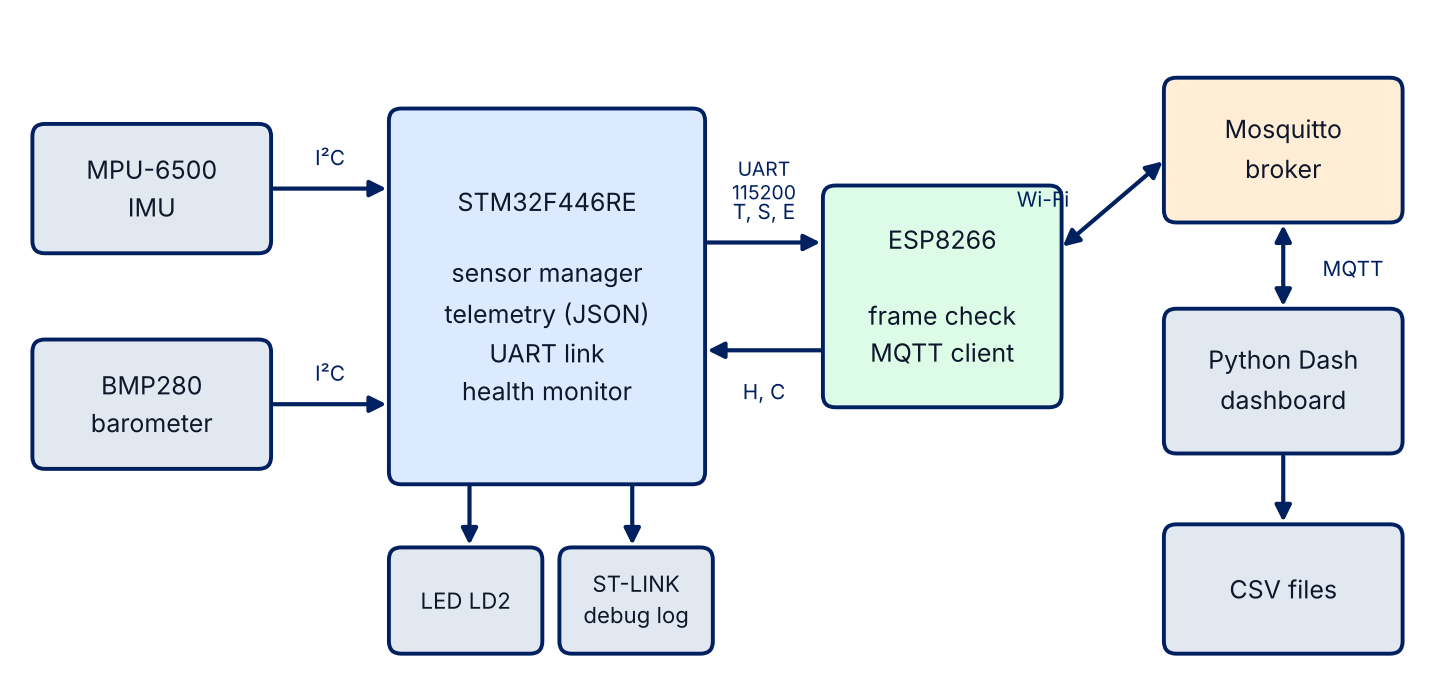
\includegraphics[width=0.95\textwidth]{img_block.png}
\caption{System block diagram of AERIS}
\label{fig:block}
\end{figure}

\section{IoT Architecture Layers}
AERIS contains the main IoT building blocks, arranged in layers:
\begin{enumerate}
\item \textbf{Perception layer:} the MPU-6500 and BMP280 sensors.
\item \textbf{Edge layer:} the STM32F446RE, which samples, filters (averaging) and packs the data.
\item \textbf{Network layer:} the UART link, the ESP8266 with Wi-Fi, and MQTT with topics, retained messages and a last-will message.
\item \textbf{Application layer:} the Dash dashboard, CSV storage and a command channel back to the device.
\end{enumerate}
Separating the measurement controller from the networking controller is a common technique in real instrumentation, because the measurement schedule must not depend on the state of the network.

\paragraph{Local broker versus cloud.} AERIS uses a local MQTT broker on the same network as the ESP8266, not a public cloud service. This keeps the data on the local network, needs no internet access and has low latency. The price is that the data is available only while the broker computer is running and reachable. A cloud-connected system can serve many users, but it needs internet access and security configuration (TLS and user accounts), and it has higher latency.

\paragraph{Proposed cloud extension (future scope).} A Mosquitto bridge can forward the \texttt{aeris/\#} topics from the local broker to a cloud broker over TLS, and a cloud dashboard with a database can store and plot the data. The device side does not change, which is an advantage of the publish-subscribe design. Figure~\ref{fig:cloud} shows this extension. It is not implemented in the present prototype.
\begin{figure}[htbp]
\centering
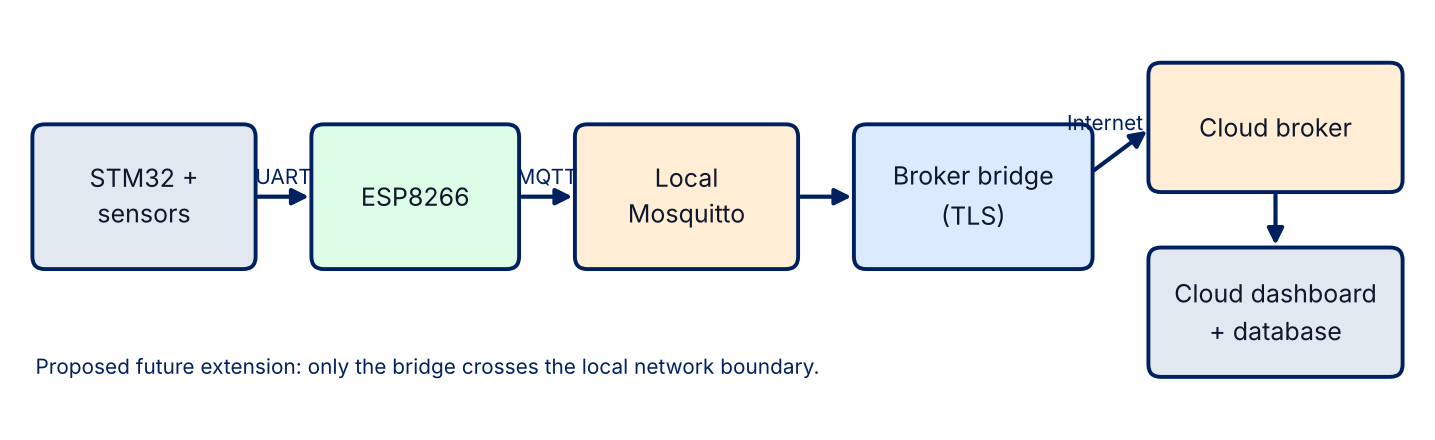
\includegraphics[width=0.95\textwidth]{img_cloud.png}
\caption{Proposed cloud-connected IoT extension (future scope)}
\label{fig:cloud}
\end{figure}

\section{Circuit Diagram}
Table~\ref{tab:wiring} specifies the point-to-point connections. The two sensors share SCL and SDA on PB8 and PB9. The UART link is crossed: PA9 (TX) goes to the ESP8266 receive pin D7 (GPIO13), and PA10 (RX) to its transmit pin D8 (GPIO15). The address pins are tied as follows: AD0 to GND and NCS to 3V3 on the MPU-6500, and SDO to GND and CSB to 3V3 on the BMP280. These ties select I$^2$C mode and a fixed address.
\begin{figure}[htbp]
\centering
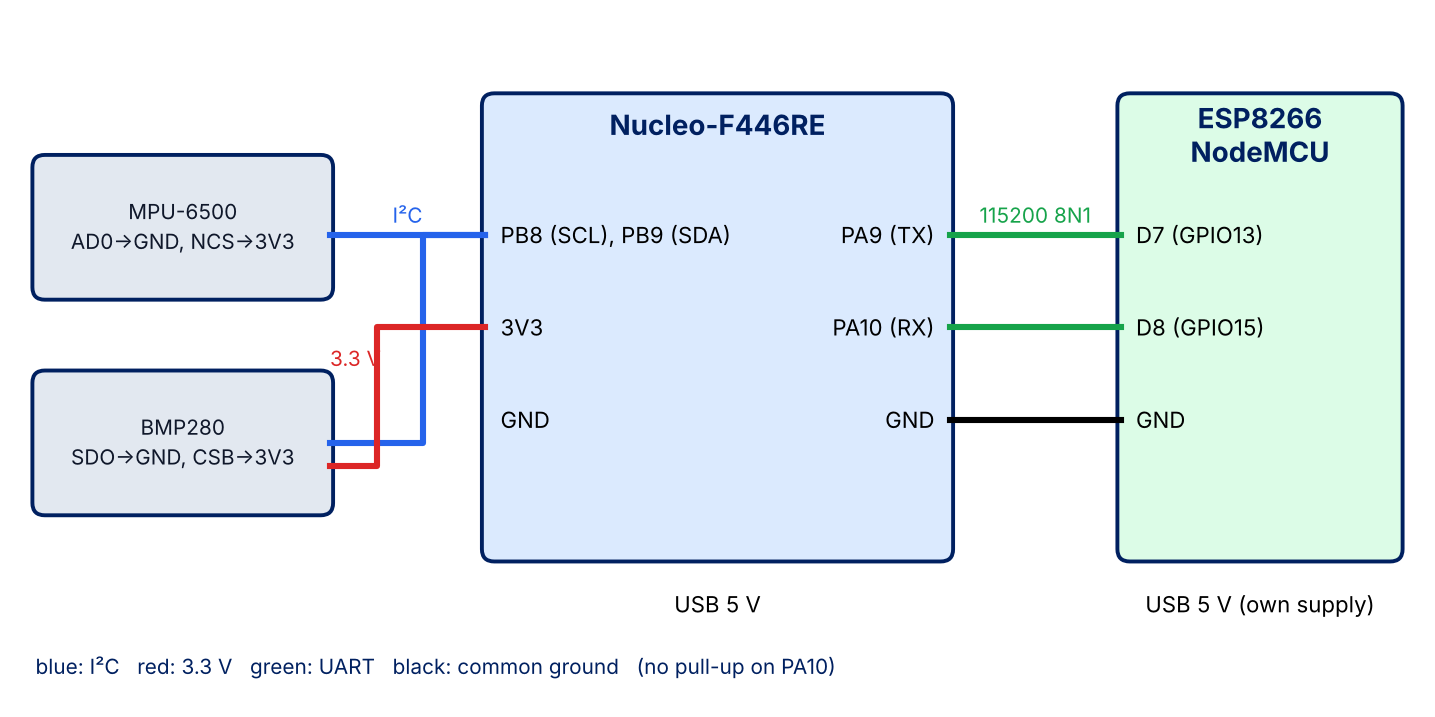
\includegraphics[width=0.95\textwidth]{img_circuit.png}
\caption{Circuit connection diagram (STM32, sensors, ESP8266)}
\label{fig:circuit}
\end{figure}

\begin{table}[htbp]
\centering
\caption{Circuit pin interconnections}
\label{tab:wiring}
\small
\begin{tabularx}{\textwidth}{>{\raggedright\arraybackslash}X>{\raggedright\arraybackslash}X>{\raggedright\arraybackslash}X>{\raggedright\arraybackslash}X}
\toprule
\textbf{Source component} & \textbf{Source pin} & \textbf{Target component} & \textbf{Target pin / wire}\\
\midrule
STM32 Nucleo & 3V3 & MPU-6500 and BMP280 & VCC (3.3 V only)\\
STM32 Nucleo & GND & Sensors and ESP8266 & GND (common ground)\\
STM32 Nucleo & PB8 (I2C1 SCL) & MPU-6500 and BMP280 & SCL\\
STM32 Nucleo & PB9 (I2C1 SDA) & MPU-6500 and BMP280 & SDA\\
STM32 Nucleo & PA9 (USART1 TX) & ESP8266 NodeMCU & D7 (GPIO13), receive\\
ESP8266 NodeMCU & D8 (GPIO15), transmit & STM32 Nucleo & PA10 (USART1 RX), no pull-up\\
Each board & USB port & Computer or USB supply & Separate 5 V USB supply per board\\
\bottomrule
\end{tabularx}
\end{table}

\section{Flowchart and Data Flow Diagram}
The operation of AERIS has five phases:
\begin{enumerate}
\item \textbf{Start-up:} The STM32 initialises the clock, the I$^2$C bus and the UARTs. Each sensor passes through the states RESET and WAIT to RUN.
\item \textbf{Sampling:} The IMU is polled every 10 ms and the barometer every 100 ms. Three read errors in a row, or a bad configuration read-back, put a sensor in FAULT, and the firmware retries once per second.
\item \textbf{Packaging:} Every 50 ms the firmware averages about five IMU samples, adds the pressure altitude and sends a T frame. Every second it sends an S frame with states and counters.
\item \textbf{Transport:} The ESP8266 checks each frame and publishes it to the broker. If the broker is not reachable, it drops telemetry and reconnects.
\item \textbf{Presentation:} The dashboard validates the message, checks the sequence number, updates the plots and, while recording, writes a CSV row.
\end{enumerate}
Figure~\ref{fig:flow} shows the main loop of the STM32 firmware. The loop never blocks for longer than one I$^2$C transfer (5 ms timeout). Each task has a deadline that advances by a fixed period, so the average rate stays correct. If the loop is late, the deadline moves to the current time, so packets are not sent in a burst.
\begin{figure}[htbp]
\centering
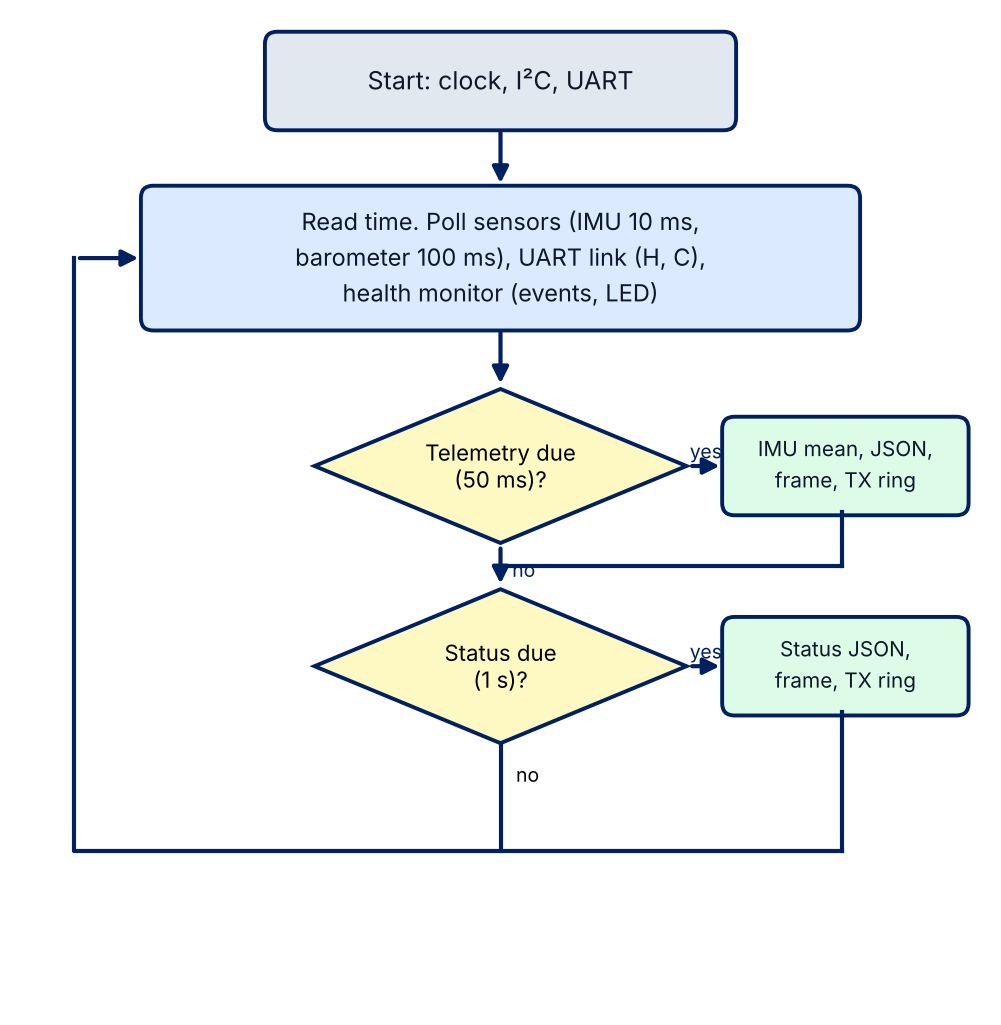
\includegraphics[width=0.62\textwidth]{img_flow.png}
\caption{STM32 main loop flowchart}
\label{fig:flow}
\end{figure}

Table~\ref{tab:dfd} gives the data flow between the processes of the system.
\begin{table}[htbp]
\centering
\caption{Data flow between the system stages}
\label{tab:dfd}
\small
\begin{tabularx}{\textwidth}{>{\raggedright\arraybackslash}p{3cm}>{\raggedright\arraybackslash}p{3.4cm}>{\raggedright\arraybackslash}p{3.2cm}X}
\toprule
\textbf{From} & \textbf{Process} & \textbf{To} & \textbf{Data}\\
\midrule
MPU-6500, BMP280 & Sampling and averaging (STM32) & Telemetry builder & Acceleration, angular rate, pressure, temperature\\
Telemetry builder & Frame with sequence number, timestamp and XOR checksum & ESP8266 (UART) & \texttt{\$T:\{json\}*HH} lines\\
ESP8266 & Frame check and MQTT publish & Mosquitto broker & Messages on \texttt{aeris/\ldots} topics\\
Mosquitto broker & Validation, plotting, recording & Dashboard, CSV file & Plots, diagnostics, CSV rows\\
Dashboard & QNH command & ESP8266, then STM32 & \texttt{aeris/command}, C frame\\
\bottomrule
\end{tabularx}
\end{table}

\section{Communication Protocol Selection}
Every message between the two controllers is one ASCII line of the form \texttt{\$K:<json>*HH}, sent at 115200 baud, 8N1. The kind letter $K$ selects the content, the JSON payload carries the values, and the two hexadecimal characters $HH$ are the XOR of all bytes between the dollar sign and the asterisk. The leading \texttt{\$} lets the receiver find the next frame after an error. The ESP8266 rejects frames with a wrong length, checksum or JSON shape.

The STM32 sends telemetry (T), status (S) and event (E) frames. The ESP8266 sends a heartbeat (H) with the Wi-Fi and MQTT state once per second and forwards commands (C) from the dashboard, for example a new QNH value. If the heartbeat stops, the STM32 shows this on its LED and keeps sampling. If MQTT is not available, the ESP8266 drops telemetry, keeps the latest status and the last eight events, and reconnects with a back-off of 1 s to 16 s.

\textbf{Why UART and MQTT.} UART frames with a checksum are simple, easy to inspect with a serial terminal and need no extra hardware between two boards. MQTT suits telemetry because publishers and subscribers are decoupled, it runs over ordinary Wi-Fi and TCP, and it offers retained and last-will messages. Figure~\ref{fig:frame} shows the frame and the topics, and Table~\ref{tab:frames} lists the frame kinds.
\begin{figure}[htbp]
\centering
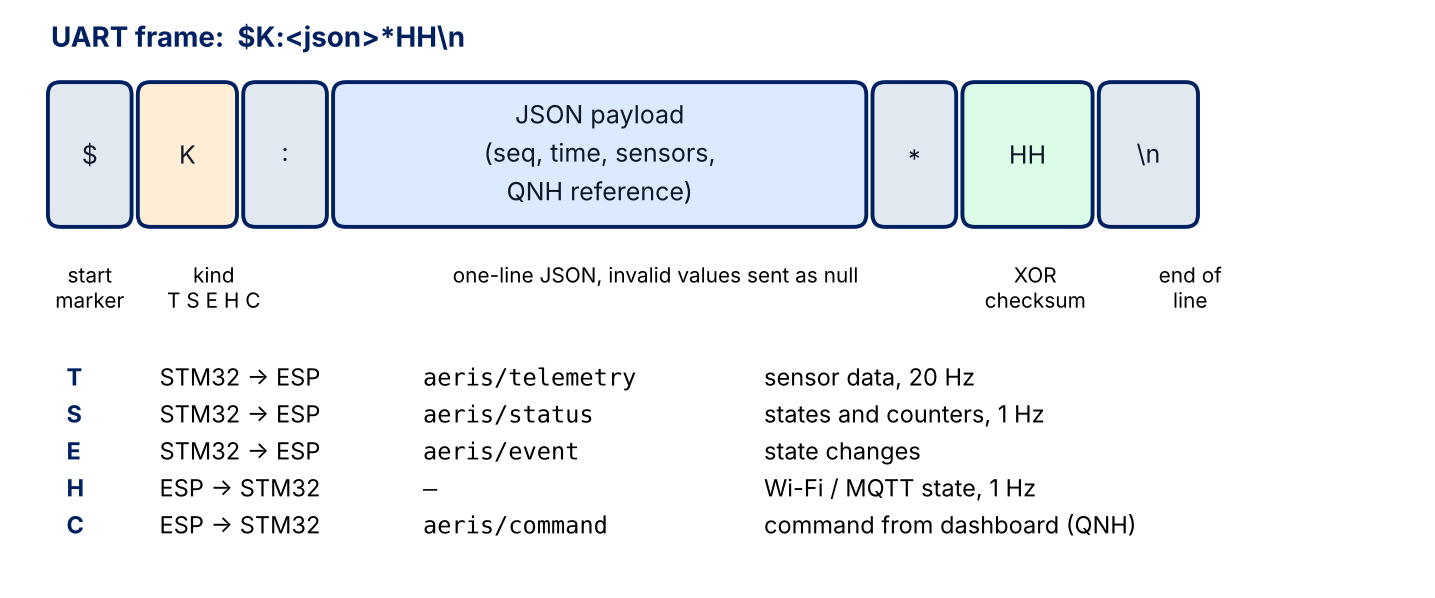
\includegraphics[width=0.95\textwidth]{img_frame.png}
\caption{UART frame format and MQTT topic mapping}
\label{fig:frame}
\end{figure}

\begin{table}[htbp]
\centering
\caption{Frame kinds and MQTT topics}
\label{tab:frames}
\small
\begin{tabularx}{\textwidth}{llllX}
\toprule
\textbf{Kind} & \textbf{Direction} & \textbf{MQTT topic} & \textbf{Rate} & \textbf{Content}\\
\midrule
T & STM32 to ESP8266 & aeris/telemetry & 20 Hz & Sensor data\\
S & STM32 to ESP8266 & aeris/status & 1 Hz & States and counters\\
E & STM32 to ESP8266 & aeris/event & On change & State changes\\
H & ESP8266 to STM32 & -- & 1 Hz & Wi-Fi and MQTT state\\
C & ESP8266 to STM32 & aeris/command & On request & Command from dashboard (QNH)\\
-- & ESP8266 to broker & aeris/status/esp & 5 s & Bridge diagnostics, retained\\
\bottomrule
\end{tabularx}
\end{table}

\section{Component Selection Rationale}
\begin{table}[htbp]
\centering
\caption{Component selection comparison (approximate prices)}
\label{tab:select}
\small
\begin{tabularx}{\textwidth}{>{\raggedright\arraybackslash}p{2.2cm}>{\raggedright\arraybackslash}p{2.8cm}>{\raggedright\arraybackslash}p{1.7cm}>{\raggedright\arraybackslash}Xl}
\toprule
\textbf{Component} & \textbf{Candidate} & \textbf{Cost} & \textbf{Power / Interface} & \textbf{Decision}\\
\midrule
Microcontroller & STM32 Nucleo-F446RE & \rupee\,2000 & 3.3 V logic, Cortex-M4F at 84 MHz, 128 KB SRAM, on-board ST-LINK & Selected\\
                & Arduino Uno & \rupee\,600 & 5 V logic, 16 MHz AVR, 2 KB SRAM & Rejected\\
IMU             & MPU-6500 module & \rupee\,300 & 3.3 V, I$^2$C, accelerometer and gyroscope & Selected\\
                & ADXL345 module & \rupee\,250 & 3.3 V, I$^2$C, accelerometer only & Rejected\\
Barometer       & BMP280 module & \rupee\,200 & 3.3 V, I$^2$C, pressure and temperature & Selected\\
                & BMP180 module & \rupee\,150 & 3.3 V, I$^2$C, older, lower resolution & Rejected\\
Comm.\ module   & ESP8266 NodeMCU & \rupee\,350 & 3.3 V, Wi-Fi and TCP/IP, UART to the STM32 & Selected\\
                & HC-05 Bluetooth & \rupee\,250 & 3.3 V logic, UART, no IP or MQTT & Rejected\\
\bottomrule
\end{tabularx}
\end{table}
The STM32 gives predictable timing, a floating-point unit and enough memory for the sampling loop and ring buffers, and its ST-LINK allows flashing and debugging without extra hardware. The MPU-6500 provides both acceleration and rotation rate, and the BMP280 provides pressure for the altitude estimate. The ESP8266 offers Wi-Fi and a ready MQTT library at a very low price. Prices are approximate market estimates.

% ---------------- CHAPTER 5 ----------------
\chapter{Hardware Description}
\section{Microcontroller}
The STM32 Nucleo-F446RE hosts the sampling firmware. It uses a Cortex-M4F core running at 84 MHz in AERIS (clock from the internal oscillator through the PLL), 512 KB flash and 128 KB SRAM. The on-board ST-LINK is used to flash the firmware and also provides a virtual COM port (USART2) for a non-blocking debug log at 115200 baud. All logic levels are 3.3 V. The firmware is bare-metal (no RTOS) and uses a cooperative, deadline-driven main loop.

\section{Sensors and Actuators}
\textbf{MPU-6500 (IMU).} Three-axis accelerometer and three-axis gyroscope on I$^2$C at 400 kHz. It is configured for $\pm$4 g and $\pm$500 deg/s with a 41 Hz digital low-pass filter and is read at 100 Hz. The firmware checks the WHO\_AM\_I register and reads back the configuration.

\textbf{BMP280 (barometer).} Pressure and die temperature on the same I$^2$C bus, with $\times$16 oversampling and IIR filter coefficient 16, read at 10 Hz. The firmware verifies the chip id and calibration data and applies plausibility limits.

\textbf{Actuator / indicator.} The AERIS prototype has no motor or relay. The only output device is the on-board LED LD2 (PA5), which shows the system state (Chapter~\ref{ch:manual}).

\section{Power Supply and Connectivity Modules}
\textbf{ESP8266 NodeMCU.} It provides Wi-Fi and the MQTT client and is connected to the STM32 by a crossed UART link. Each board has its own USB supply, because the ESP8266 draws current peaks of about 300 mA and the Nucleo 3V3 pin is not meant to power it.

\textbf{Electrical safety.}
\begin{itemize}
\item All signals are 3.3 V, so 5 V must never be connected to a sensor or a GPIO pin.
\item GPIO15 of the ESP8266 must be low when the board starts, so no pull-up resistor may be placed on PA10.
\item Both boards must share a common ground.
\item Disconnect USB before the wiring is changed.
\end{itemize}

\section{Pin Configuration}
\begin{table}[htbp]
\centering
\caption{Pin mapping of the STM32 Nucleo-F446RE}
\label{tab:pins}
\small
\begin{tabularx}{\textwidth}{llXl}
\toprule
\textbf{MCU Pin} & \textbf{Connected To} & \textbf{Function} & \textbf{Voltage}\\
\midrule
PB8 & MPU-6500 and BMP280 SCL & I$^2$C1 clock (400 kHz) & 3.3 V\\
PB9 & MPU-6500 and BMP280 SDA & I$^2$C1 data & 3.3 V\\
PA9 & ESP8266 D7 (GPIO13) & USART1 TX: telemetry, status and event frames out & 3.3 V\\
PA10 & ESP8266 D8 (GPIO15) & USART1 RX: heartbeat and command frames in (no pull-up) & 3.3 V\\
PA5 & LED LD2 & System status indicator & 3.3 V\\
3V3 / GND & Sensor power / common ground & 3.3 V supply and common reference & 3.3 V\\
\bottomrule
\end{tabularx}
\end{table}

\section{Bill of Materials (BOM)}
\begin{table}[htbp]
\centering
\caption{Bill of Materials (prices are approximate estimates)}
\label{tab:bom}
\small
\begin{tabularx}{\textwidth}{llXlrrl}
\toprule
\textbf{S.No} & \textbf{Ref.} & \textbf{Description / Part No.} & \textbf{Qty} & \textbf{Unit (\rupee)} & \textbf{Total (\rupee)} & \textbf{Supplier}\\
\midrule
1 & U1 & STM32 Nucleo-F446RE development board & 1 & 2000 & 2000 & Online / local\\
2 & U2 & ESP8266 NodeMCU Wi-Fi module & 1 & 350 & 350 & Online / local\\
3 & S1 & MPU-6500 IMU breakout & 1 & 300 & 300 & Online / local\\
4 & S2 & BMP280 barometer breakout & 1 & 200 & 200 & Online / local\\
5 & W1 & Breadboard & 1 & 100 & 100 & Online / local\\
6 & W2 & Jumper wires (DuPont set) & 1 & 80 & 80 & Online / local\\
7 & P1 & USB cables (Mini-B and Micro-B) & 2 & 100 & 200 & Online / local\\
\midrule
\multicolumn{5}{r}{\textbf{Total project cost}} & \textbf{3230} & \\
\bottomrule
\end{tabularx}
\end{table}

\section{Power Budget}
The values in Table~\ref{tab:power} are typical datasheet or approximate figures, not measurements. AERIS is powered from USB, and the budget is given to show what a battery version would need.
\begin{table}[htbp]
\centering
\caption{Power budget (typical values, not measured)}
\label{tab:power}
\renewcommand{\arraystretch}{1.6}
\setlength{\tabcolsep}{8pt}
\begin{tabularx}{\textwidth}{>{\raggedright\arraybackslash}X
    >{\centering\arraybackslash}p{1.8cm}
    >{\centering\arraybackslash}p{1.8cm}
    >{\centering\arraybackslash}p{1.8cm}
    >{\centering\arraybackslash}p{1.8cm}}
\toprule
\textbf{Component} & \textbf{Voltage}\newline(V) & \textbf{Active}\newline(mA) & \textbf{Sleep}\newline(mA) & \textbf{Duty}\newline(\%)\\
\midrule
STM32F446RE (84 MHz, peripherals) & 3.3 & 30 & -- & 100\\
MPU-6500 (gyro and accelerometer) & 3.3 & 3.7 & -- & 100\\
BMP280 ($\times$16, 10 Hz) & 3.3 & 0.05 & -- & 100\\
ESP8266 (Wi-Fi connected, average) & 3.3 & 80 & -- & 100\\
\midrule
\textbf{Total} & 3.3 & \textbf{113.75} & -- & --\\
\bottomrule
\end{tabularx}
\end{table}

\vspace{0.3cm}
\noindent\textbf{Average current:} about 114 mA (all components run continuously; ESP8266 peaks of about 300 mA are not included).

\vspace{0.2cm}
\noindent\textbf{Estimated battery life} $=$ battery capacity (mAh) $\div$ average current (mA). For an illustrative 2000 mAh battery: $2000 \div 113.75 \approx 17.6$ hours (ideal, without regulator losses).

% ---------------- CHAPTER 6 ----------------
\chapter{Software Implementation}
\section{Tools and IDEs Used}
The software stack uses open-source tools (Table~\ref{tab:sw}). The STM32 firmware is written in C with the STM32 HAL in STM32CubeIDE and does not use an RTOS. The ESP8266 sketch is built in the Arduino IDE with the ESP8266 core 3.1.2 and the PubSubClient 2.8 library. On the computer, Mosquitto is the MQTT broker, and a Python application with Dash, Plotly and paho-mqtt provides the dashboard and the CSV recorder. A pytest suite tests validation, sequence tracking, the recorder and the MQTT path.

\section{Algorithm and Logic}
\begin{enumerate}
\item \textbf{Initialise:} Set up the clock, I$^2$C1 (400 kHz), USART1 (115200 8N1) and the debug USART2.
\item \textbf{Start sensors:} Move the MPU-6500 and BMP280 through RESET and WAIT into RUN and verify their configuration by read-back.
\item \textbf{Poll (loop):} Read the time and poll the sensor manager, the UART link and the health monitor without blocking.
\item \textbf{Telemetry due (every 50 ms):} Average the IMU samples, compute the pressure altitude, build the JSON, add the XOR checksum and put the frame in the TX ring buffer.
\item \textbf{Status due (every 1 s):} Build the status JSON and queue it in the same way.
\item \textbf{Handle commands:} On a C frame, set the new QNH and report the result as an event.
\item \textbf{Repeat} without blocking delays. A full TX buffer drops the new frame instead of waiting.
\end{enumerate}

\textbf{Sampling, averaging and altitude.} Each telemetry packet carries the mean of about five IMU samples (100 Hz reduced to 20 Hz). This lowers random noise by roughly a factor of 2.2 (the square root of 5). The barometer is updated at 10 Hz, so its fields can be up to 100 ms older than the IMU fields, and each carries its own timestamp. If a sensor is in FAULT, or the barometer reading is older than 500 ms, the corresponding values are sent as \texttt{null}, so the dashboard shows a gap and not a false zero. The device time is the time since boot and wraps after about 49.7 days; the host receive time is recorded separately in the CSV file.

\section{Key Code Snippets}
The listing below is the main loop of the STM32 firmware (\texttt{aeris\_app.c}) from the AERIS repository~\cite{aeris}. It shows the non-blocking polling and the fixed-period telemetry deadline.
\begin{lstlisting}[language=C,caption={STM32 main loop (aeris\_app.c, from the AERIS repository)}]
void aeris_app_loop(void)
{
    uint32_t now = timebase_ms();
    sensor_manager_poll(now);   /* IMU, barometer */
    uart_link_poll(now);        /* H and C frames */
    health_monitor_poll(now, telemetry_dropped);

    if (timebase_reached(now, next_telemetry_ms)) {
        next_telemetry_ms += TELEMETRY_PERIOD_MS;
        if (timebase_reached(now, next_telemetry_ms))
            next_telemetry_ms = now + TELEMETRY_PERIOD_MS;
        send_telemetry(now);    /* JSON, frame, TX ring */
    }
    /* status (1 s): same pattern */
}
\end{lstlisting}

\section{Cloud / Dashboard / App Setup}
AERIS uses a local broker and a local dashboard. The set-up has four steps.
\begin{enumerate}
\item \textbf{Broker (Ubuntu).} Install Mosquitto, copy \texttt{docs/mosquitto/aeris.conf} to \texttt{/etc/mosquitto/conf.d/}, create the password file with \texttt{mosquitto\_passwd}, and restart the service. The listener on port 1883 is password protected and for the local network only.
\item \textbf{Dashboard.} Create a Python virtual environment, run \texttt{pip install -r requirements.txt}, enter the broker user name and password in \texttt{config.yaml}, and start \texttt{python dashboard/app.py}. Open \texttt{http://127.0.0.1:8050}.
\item \textbf{Simulator (optional).} Run \texttt{python tools/simulate\_device.py --loss 0.01 --invalid 0.005 --pause-at 30} to publish synthetic telemetry without hardware.
\item \textbf{ESP8266.} Edit \texttt{config.h} (Wi-Fi name and password, broker IP address, MQTT user and password), then upload the sketch from the Arduino IDE.
\end{enumerate}
The dashboard shows the device ID, the state CONNECTED, STALE or DISCONNECTED, five live plots (acceleration, angular rate, pressure, temperature and altitude), diagnostics (sequence, missing, duplicate and out-of-order packets, reboots, invalid messages), the STM32 and ESP8266 states, and the recorder state. A QNH control sends the \texttt{set\_sea\_level\_hpa} command to the STM32.

% ---------------- CHAPTER 7 ----------------
\chapter{Testing, Results and Risk Analysis}
\label{ch:testing}
\section{Test Cases}
Testing has two stages. \textbf{Stage 1 (completed)} used the device simulator \texttt{tools/simulate\_device.py}, which publishes synthetic telemetry with a chosen packet-loss rate and invalid-message rate. It tested the broker, the dashboard and the CSV recorder without hardware, and was started with \texttt{--loss 0.01 --invalid 0.005 --pause-at 30}. \textbf{Stage 2 (pending)} repeats the tests with the real STM32 and ESP8266 hardware on a 2.4 GHz phone hotspot network and fills the entries marked [to be filled].

Table~\ref{tab:tests} lists the test cases. Entries marked \textbf{Pending} have not been measured yet and must not be read as passed.

{\footnotesize
\setlength{\tabcolsep}{3pt}
\begin{longtable}{>{\raggedright\arraybackslash}p{0.9cm}>{\raggedright\arraybackslash}p{0.9cm}>{\raggedright\arraybackslash}p{3.2cm}>{\raggedright\arraybackslash}p{2.7cm}>{\raggedright\arraybackslash}p{4.1cm}>{\raggedright\arraybackslash}p{1.5cm}}
\caption{Test cases and results}\label{tab:tests}\\
\toprule
\textbf{Test ID} & \textbf{Req ID} & \textbf{Procedure} & \textbf{Expected} & \textbf{Actual} & \textbf{Result}\\
\midrule
\endfirsthead
\toprule
\textbf{Test ID} & \textbf{Req ID} & \textbf{Procedure} & \textbf{Expected} & \textbf{Actual} & \textbf{Result}\\
\midrule
\endhead
\bottomrule
\endfoot
T1 & R9 & Broker login with a wrong and then the correct password & Wrong password rejected, correct accepted & ``not authorised'' for the wrong password; accepted for user \texttt{aeris} & Pass\\
T2 & R3 & Dashboard with simulator running & Header CONNECTED, live plots & CONNECTED, device \texttt{aeris-sim}, last message 51 ms old & Pass\\
T3 & R4 & Simulator with 0.5\,\% invalid packets & Invalid packets rejected, not plotted & 12 rejected; last reason: non-finite JSON constant NaN & Pass\\
T4 & R5 & Simulator with 1\,\% loss and a pause at 30 s & Missing counter rises, no duplicates & Missing 144; duplicates 0; out of order 0; reboots 0 & Pass\\
T5 & R6 & Start and stop CSV recording & CSV file with rows, none dropped & 104 rows written, 0 dropped, file saved in the data folder & Pass\\
T6 & R7 & QNH sent from the dashboard & Command sent; acknowledgement event from device & Command sent (1013.25 hPa); acknowledgement needs hardware & Pending\\
T7 & R2, R3 & ESP8266 on phone hotspot with real STM32 & Header CONNECTED with the real device ID & [to be filled] & Pending\\
T8 & R2, R10 & 20 Hz for 10 min on hardware & Packet loss below 1\,\% & [to be filled] & Pending\\
T9 & R1 & Unit level and still & Acceleration magnitude about 1 g & [to be filled] & Pending\\
T10 & R4, R5 & Run the pytest suite & All tests pass & [to be filled after running pytest] & Pending\\
T11 & R8 & Switch the Wi-Fi hotspot off for 30 s while hardware runs & STM32 sampling and LED continue; frames resume after reconnect & [to be filled] & Pending\\
\end{longtable}
}

\section{Screenshots and Performance Results}
Figures~\ref{fig:dash1} to~\ref{fig:dash3} are dashboard screenshots from the simulator run on 21 October 2026. The values are synthetic and show the behaviour of the software chain only; they are not sensor measurements. The dashboard counters were: received 2395, accepted 2383, invalid 12, missing (sequence gaps) 144, duplicates 0, out of order 0 and reboots 0. The recorder wrote 104 rows to \texttt{aeris\_2026-10-21\_20-56-22.csv} with 0 dropped. The missing count is expected to include gaps from the injected loss, from rejected packets and from the deliberate pause at 30 s.

\begin{figure}[htbp]
\centering
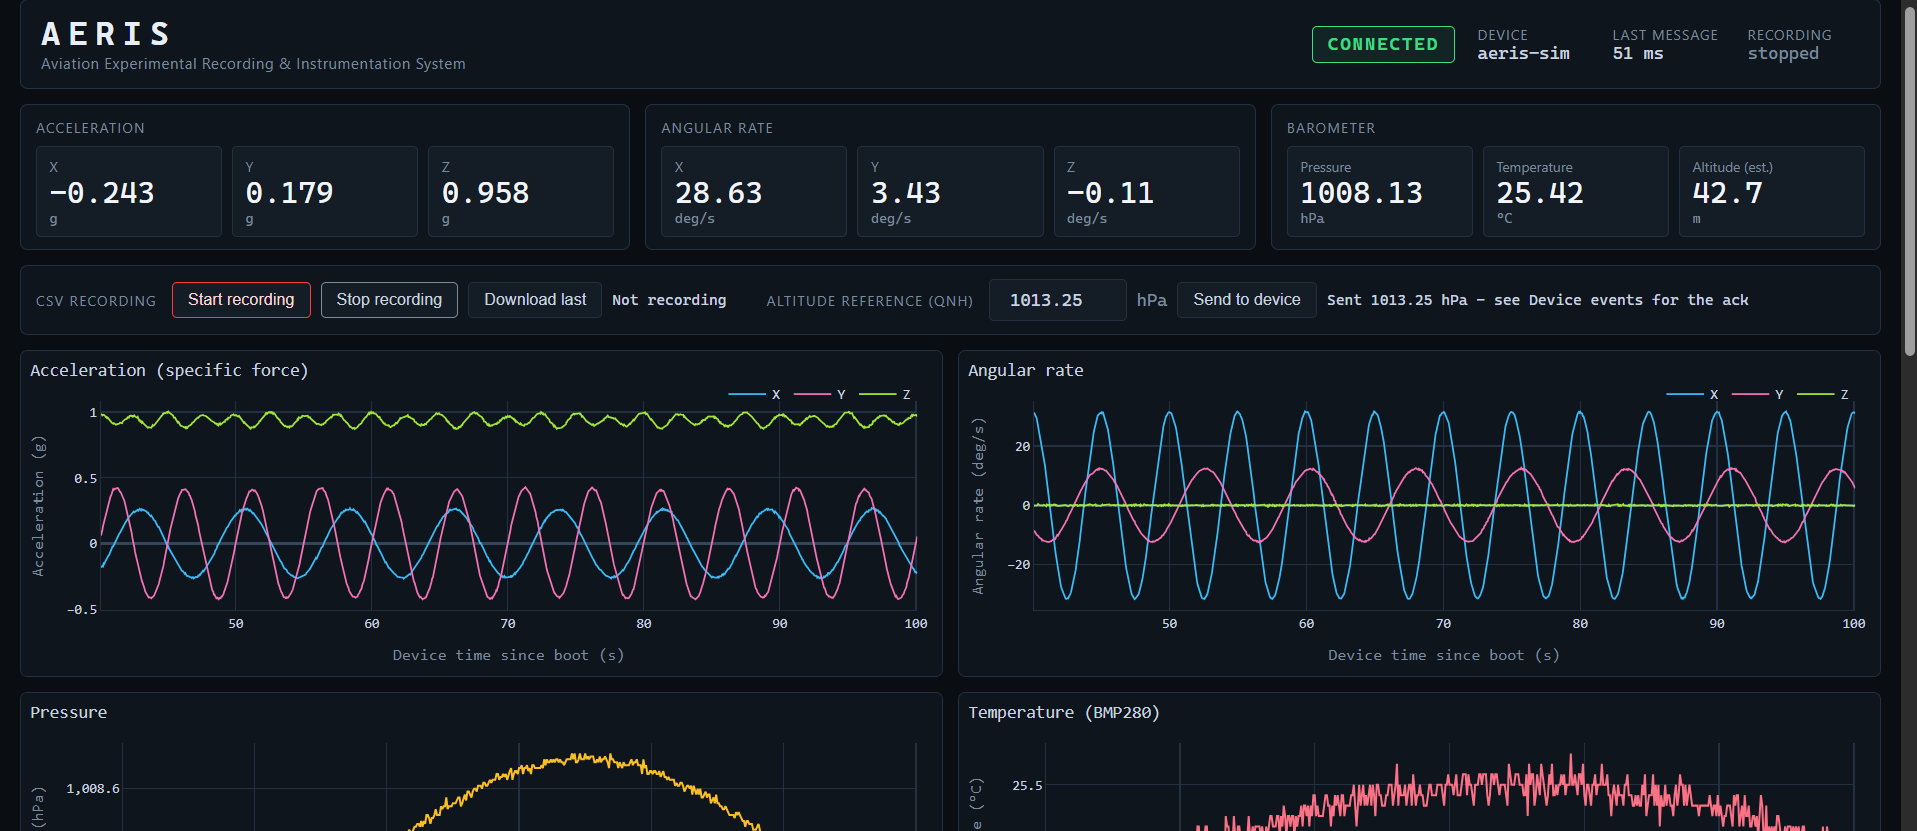
\includegraphics[width=\textwidth]{img_dash1.png}
\caption{Dashboard live view during the simulator run}
\label{fig:dash1}
\end{figure}
\begin{figure}[htbp]
\centering
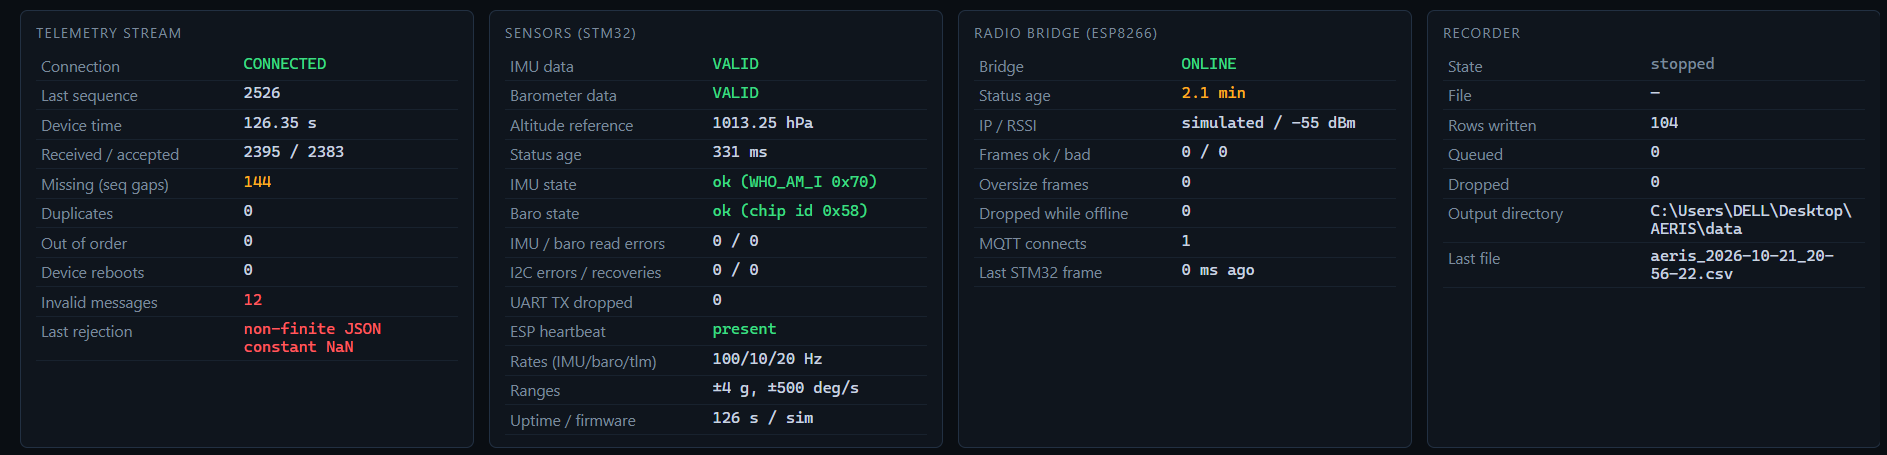
\includegraphics[width=\textwidth]{img_dash2.png}
\caption{Diagnostics panels (telemetry, sensors, radio bridge, recorder)}
\label{fig:dash2}
\end{figure}
\begin{figure}[htbp]
\centering
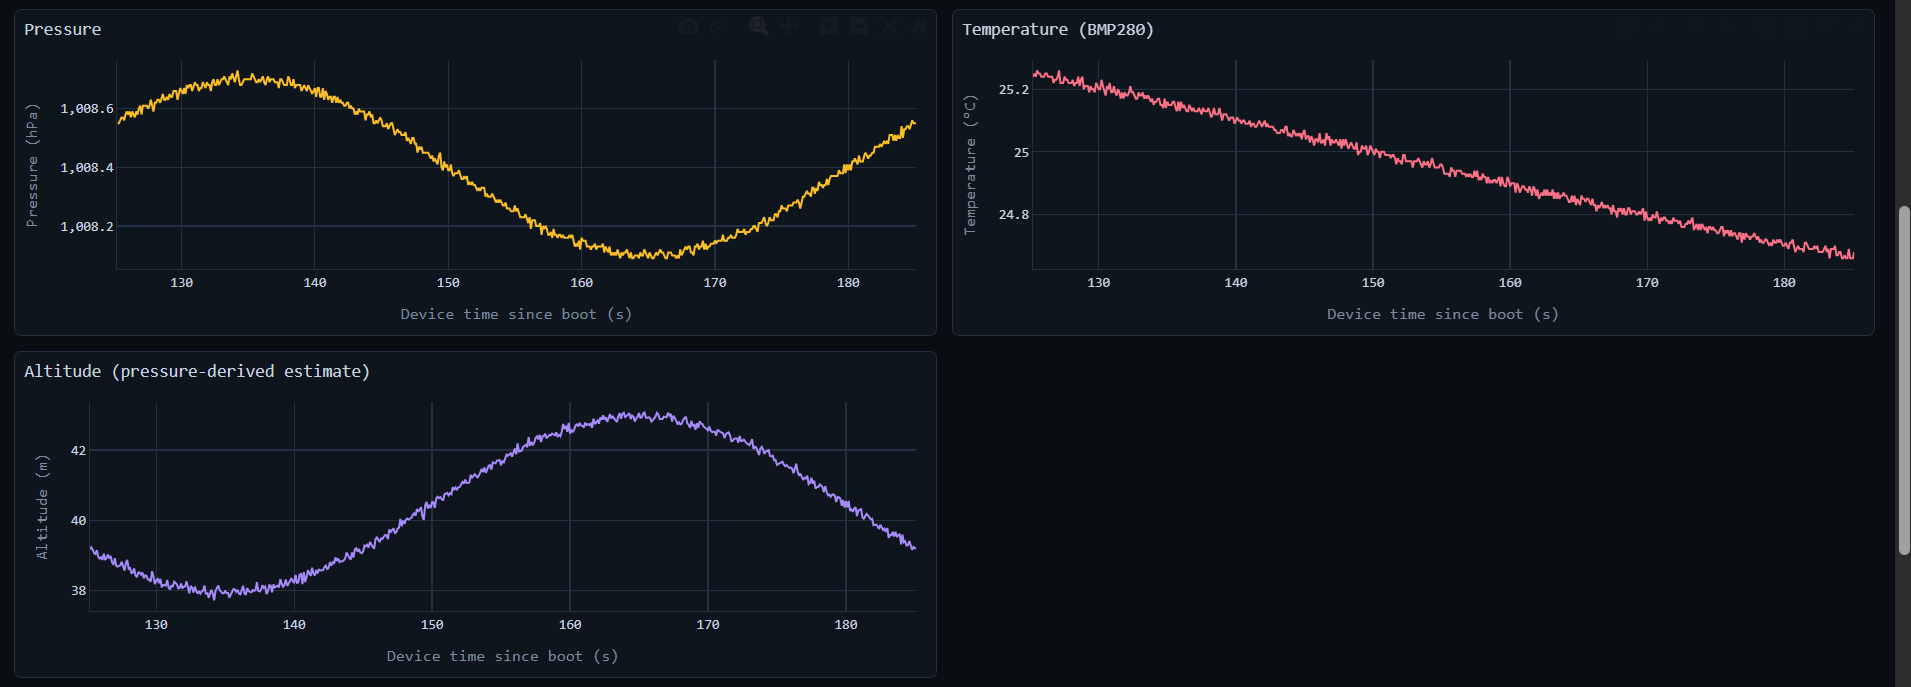
\includegraphics[width=\textwidth]{img_dash3.png}
\caption{Pressure, temperature and altitude plots (simulator data)}
\label{fig:dash3}
\end{figure}

\section{Risk Analysis}
\begin{table}[htbp]
\centering
\caption{Risk analysis}
\label{tab:risk}
\small
\begin{tabularx}{\textwidth}{lXllX}
\toprule
\textbf{ID} & \textbf{Risk} & \textbf{Likelihood} & \textbf{Impact} & \textbf{Mitigation}\\
\midrule
K1 & Wi-Fi connection loss & Medium & High & ESP8266 reconnects with 1--16 s back-off; STM32 keeps sampling; gaps are visible in sequence numbers\\
K2 & Sensor drift / failure & Low & Medium & Per-sensor state machine (FAULT, retry every 1 s); invalid values sent as \texttt{null}; fault events on the dashboard\\
K3 & Power failure & Medium & High & Separate USB supply per board; battery and regulator listed as future work\\
K4 & I$^2$C bus lock-up & Low & High & 5 ms transfer timeouts and bus recovery in firmware\\
K5 & Wrong or reset QNH gives an altitude offset & Medium & Medium & QNH stored in every packet and CSV row; resend QNH from the dashboard after a reboot\\
K6 & 5 V connected to a 3.3 V pin & Low & High & All parts run at 3.3 V; safety notes in Chapter~\ref{ch:manual}; disconnect USB before rewiring\\
K7 & Broker computer off or unreachable & Medium & High & Dashboard shows STALE or DISCONNECTED; run the broker on a computer that stays on during tests\\
\bottomrule
\end{tabularx}
\end{table}

\section{Challenges Faced and Solutions}
\begin{table}[htbp]
\centering
\caption{Challenges and solutions}
\label{tab:chal}
\small
\begin{tabularx}{\textwidth}{>{\raggedright\arraybackslash}p{5.2cm}X}
\toprule
\textbf{Challenge} & \textbf{Solution}\\
\midrule
The complete hardware set was not available for testing during the project period & Tested the software chain with the device simulator first and marked the hardware tests as Pending instead of reporting unmeasured results\\
Wi-Fi reconnection can delay sensor reads when one controller does everything & Split the work: STM32 samples on a fixed schedule, ESP8266 handles networking only\\
A failed sensor can look like valid data (reading of zero) & Invalid values travel as \texttt{null} and are shown as gaps and dashes\\
ESP8266 needs GPIO15 low at boot and draws current peaks of about 300 mA & No pull-up on PA10; separate USB supply for the ESP8266\\
Packet loss and bit errors on the link & Sequence numbers, timestamps and XOR checksum on every frame; the dashboard counts missing, duplicate and out-of-order packets\\
\bottomrule
\end{tabularx}
\end{table}

% ---------------- CHAPTER 8 ----------------
\chapter{User Manual}
\label{ch:manual}
\begin{center}
\collegelogo{1.6cm}
\end{center}
\noindent\textbf{Product name:} \projecttitle

\section*{1. What the device does}
AERIS records acceleration, rotation rate, pressure, temperature and an estimated altitude, sends them over Wi-Fi to a computer, and shows them live on a web dashboard. It can also save the data to a CSV file. It is a laboratory demonstrator and not a certified aircraft instrument.

\section*{2. What is in the box}
STM32 Nucleo-F446RE board; ESP8266 NodeMCU board; MPU-6500 and BMP280 sensor modules; breadboard and jumper wires; two USB cables. A computer with Mosquitto, Python and the dashboard software is also needed.

\section*{3. Powering on}
Wire the boards as shown in Figure~\ref{fig:circuit} and Table~\ref{tab:wiring}. Check that there is a common ground and that nothing at 5 V touches a sensor or signal pin. Connect each board to its own USB supply. The ESP8266 should be powered first if it fails to boot.

\section*{4. Connecting to the network / app}
Start the Mosquitto broker on the computer. Set the Wi-Fi name, Wi-Fi password and the computer's local IP address in the ESP8266 \texttt{config.h} and upload the sketch. Start the dashboard with \texttt{python dashboard/app.py} and open \texttt{http://127.0.0.1:8050}. The header shows CONNECTED when data arrives. Use Start and Stop to record a CSV file in the \texttt{data} folder, and the QNH control to set the altitude reference.

\section*{5. LED indicators}
\begin{center}
\begin{tabular}{ll}
\toprule
\textbf{LD2 state (STM32)} & \textbf{Meaning}\\
\midrule
Solid on & Both sensors OK and ESP8266 heartbeat present\\
Blinking 2 Hz & Sensors are still initialising\\
Blinking 1 Hz & At least one sensor is faulted\\
Blinking 5 Hz & Sensors OK, but the ESP8266 link is lost\\
\bottomrule
\end{tabular}
\end{center}

\section*{6. Troubleshooting}
\begin{itemize}
\item \textbf{Dashboard shows DISCONNECTED or STALE:} check that Mosquitto is running, that the IP address in \texttt{config.h} is the computer's local address (not \texttt{localhost}), and that the user name and password match.
\item \textbf{LD2 blinks at 5 Hz:} the ESP8266 heartbeat is missing; check the UART wires (PA9 to D7, PA10 to D8), the common ground and the power of the ESP8266.
\item \textbf{LD2 blinks at 1 Hz:} a sensor is faulted; check the I$^2$C wires (keep them short) and the 3.3 V supply.
\item \textbf{ESP8266 does not boot:} GPIO15 must be low at start-up; power the ESP8266 first or use a 1 k$\Omega$ series resistor.
\item \textbf{Altitude looks wrong:} set the correct QNH; it returns to 1013.25 hPa after every STM32 reset.
\item \textbf{Gaps in plots:} the values were invalid or packets were lost; see the diagnostics counters.
\end{itemize}

\section*{7. Safety notes}
Use 3.3 V only for sensors and signals. Do not connect 5 V to any sensor or GPIO pin. Share a common ground between the boards. Disconnect USB before changing the wiring. Do not forward the broker port 1883 to the internet. AERIS is not certified and must not be used for real flight decisions.

% ---------------- CHAPTER 9 ----------------
\chapter{Conclusion and Future Scope}
\section{Summary of Achievements}
The project entitled ``AERIS: Aviation Experimental Recording and Instrumentation System'' demonstrates the complete data path of a flight-test instrument on a low-cost platform: two I$^2$C sensors, an STM32 sampling controller, an ESP8266 MQTT bridge, a Mosquitto broker and a Python dashboard with CSV recording. We installed and ran the broker and the dashboard, tested them with a device simulator, and verified broker authentication, rejection of invalid packets, detection of sequence gaps and CSV recording (Chapter~\ref{ch:testing}). The hardware tests with the STM32 and ESP8266 boards are listed in Table~\ref{tab:tests} and will complete the evaluation.

\textbf{Advantages and educational value.}
\begin{itemize}
\item \textbf{Visible data path:} every stage from the sensor register to the CSV row can be inspected.
\item \textbf{Fault visibility:} counters for missing, duplicate and out-of-order packets, reboots and invalid messages.
\item \textbf{Timing isolation:} sampling on the STM32 does not depend on Wi-Fi or MQTT.
\item \textbf{Low cost and open design:} hobby-grade modules and open software.
\item \textbf{Testable without hardware:} a simulator and a pytest suite check the software chain.
\end{itemize}

\textbf{Application potential.} The same architecture applies to data recorders for drones, model aircraft and model rockets, motion loggers for ground vehicles and test rigs, and teaching laboratories for sensors and IoT. It can also be the base for later work on sensor fusion and telemetry protocols.

\section{Limitations}
\label{sec:limitations}
AERIS is a demonstrator, and its limits should be understood:
\begin{itemize}
\item \textbf{Averaged IMU data:} each packet carries the mean of about five samples, not the individual 100 Hz samples.
\item \textbf{Data loss when offline:} telemetry produced while Wi-Fi or MQTT is down is dropped and shows as gaps. There is no on-device storage.
\item \textbf{Link rate:} the 115200 baud UART limits telemetry to about 20 Hz.
\item \textbf{Altitude accuracy:} altitude is a pressure-derived estimate that depends on the QNH, which returns to 1013.25 hPa after a reboot. Indoor pressure changes can cause errors of a metre or more. The BMP280 temperature is the die temperature.
\item \textbf{Not implemented:} roll, pitch, heading, gyroscope bias calibration and a watchdog.
\item \textbf{Dashboard server:} the dashboard runs on Flask's development server and is meant for single-user lab work.
\item \textbf{Hardware evidence:} the hardware tests T6 to T11 are still pending.
\end{itemize}

\section{Future Enhancements}
\begin{itemize}
\item \textbf{Attitude estimation:} gyroscope bias calibration at start-up and a complementary filter to estimate roll and pitch; a magnetometer (for example an MPU-9250) for heading; a hardware watchdog to restart the STM32 if the main loop stops.
\item \textbf{Faster link:} raise the UART speed to 460800 baud to send raw 100 Hz samples.
\item \textbf{Local storage:} add a microSD card so that data is kept while the network is down.
\item \textbf{Battery operation:} add a battery and a regulator for tests away from the bench.
\item \textbf{Security and cloud:} use TLS and per-device credentials on the broker, and bridge to a cloud broker (Figure~\ref{fig:cloud}).
\item \textbf{Persistent QNH:} store the QNH in non-volatile memory so that it survives a reboot.
\end{itemize}

% ============================================================
%  BACK MATTER
% ============================================================
\begin{thebibliography}{99}
\addcontentsline{toc}{chapter}{References}
\bibitem{ardupilot} ArduPilot Development Team, ``ArduPilot Documentation,'' [Online]. Available: https://ardupilot.org
\bibitem{mqtt} OASIS, ``MQTT Version 3.1.1,'' OASIS Standard, 2014. [Online]. Available: https://docs.oasis-open.org/mqtt/mqtt/v3.1.1/mqtt-v3.1.1.html
\bibitem{stm32} STMicroelectronics, ``STM32F446xC/E Datasheet,'' DS10693. [Online]. Available: https://www.st.com
\bibitem{mpu6500} TDK InvenSense, ``MPU-6500 Product Specification,'' Doc.\ PS-MPU-6500A-01.
\bibitem{bmp280} Bosch Sensortec, ``BMP280 Digital Pressure Sensor Datasheet,'' BST-BMP280-DS001.
\bibitem{esp8266} Espressif Systems, ``ESP8266EX Datasheet.'' [Online]. Available: https://www.espressif.com
\bibitem{mosquitto} Eclipse Mosquitto, ``Mosquitto MQTT Broker Documentation,'' [Online]. Available: https://mosquitto.org
\bibitem{aeris} A.\ Kumar and A.\ S.\ Parihar, ``AERIS: Aviation Experimental Recording \& Instrumentation System,'' GitHub repository Quixotic1762/AERIS, [Online]. Available: https://github.com/Quixotic1762/AERIS (accessed 21 Oct.\ 2026).
\end{thebibliography}

% ---------------- APPENDIX ----------------
\appendix
\chapter{Viva Voce Questions and Glossary}
\section{Viva Voce Questions and Concise Answers}
\noindent\textbf{Q1. What is the purpose of the checksum in the UART frame?}\\
The checksum is the XOR of the bytes between the \texttt{\$} and the \texttt{*}. The ESP8266 calculates it again and drops the frame if the value is different, so a bit error on the wire never becomes a wrong reading on the dashboard.

\medskip\noindent\textbf{Q2. Why does AERIS use two microcontrollers?}\\
The STM32 samples on a fixed schedule and does not depend on the network. The ESP8266 handles Wi-Fi and MQTT. A Wi-Fi reconnection can delay the ESP8266 but cannot change the sample timing on the STM32.

\medskip\noindent\textbf{Q3. What is QNH and why does the altitude depend on it?}\\
QNH is the sea-level reference pressure ($p_0$) in the barometric formula. The BMP280 measures only pressure, so the altitude is calculated from $p$ and $p_0$. A wrong QNH shifts the altitude. AERIS starts at 1013.25 hPa after every reset.

\medskip\noindent\textbf{Q4. Why are invalid values sent as null and not as 0?}\\
Zero is a valid reading and would hide a sensor fault. A null is shown as a gap in the plots and as a dash in the readouts, so the fault is visible.

\medskip\noindent\textbf{Q5. How is AERIS different from a commercial FTI system or a Pixhawk?}\\
Commercial systems are certified, faster and closed. A Pixhawk is a complete flight controller. AERIS is a small, open demonstrator that is not certified and isolates the sensor-to-display data path for study.

\section{Glossary of Key Technical Terms}
\begin{itemize}
\item \textbf{IMU (Inertial Measurement Unit):} a sensor package with accelerometers and gyroscopes (here the MPU-6500).
\item \textbf{QNH:} the sea-level reference pressure used to calculate pressure altitude from the measured pressure.
\item \textbf{MQTT:} a publish-subscribe messaging protocol over TCP in which messages go to named topics on a broker.
\item \textbf{XOR checksum:} an error-check value formed by the XOR of all bytes of a frame; here the two-character HH field.
\item \textbf{I$^2$C:} a two-wire serial bus (SCL and SDA) that connects the two sensors to the STM32.
\item \textbf{UART:} the asynchronous serial link between the STM32 and the ESP8266 (115200 baud, 8N1).
\end{itemize}

\end{document}
